\chapter{Расчет излучения источников}\label{radiation}
FAINA позволяет рассчитывать электромагнитное излучение от источников с заданными функциями распределения излучающих частиц и другими параметрами. Построены модели следующих типов излучения: синхротронного, обратного комптоновского рассеяния, пионного распада в результате свободно-свободного взаимодействия протонов и тормозного излучения.
\section{Функции распределения частиц}
Важнейшими исходными данными для расчета любого типа излучения является функция распределения излучающих частиц. В коде FAINA для представления распределений используется абстрактный класс ParticleDistribution и семейство наседованных от него классов, соответствующих различным конкретным реализациям. Класс ParticleDistribution имеет следующие доступные методы, описанные в Таблице \ref{ParticleDistribution}:
	\begin{table}
	\begin{center}
		\caption{Публичные методы класса ParticleDistribution }
		\label{ParticleDistribution}
		\begin{small}
		\begin{tabularx}{\textwidth}{|X|X|}
			\hline
			\textbf{ParticleDistribution} & \\
			\hline
			distribution(const double\& energy, const double\& mu, const double\& phi) & возвращает функцию распределения от энергии, косинуса полярного угла и азимутального угла, нормированную на единицу \\
			\hline
			distributionNormalized(const double\& energy, const double\& mu, const double\& phi) & возвращает функцию распределения от энергии, косинуса полярного угла и азимутального угла, нормированную на концентрацию \\
			\hline
			getConcentration() & возвращает концентрацию частиц\\
			\hline
		\end{tabularx}
	    \end{small}
	\end{center}
\end{table}

Для вычисления излучения необходимо в первую очередь задать распределение излучающих частиц. Для это нужно создать объект из подходящего класса-наследника ParticleDistribution. Дерево наследования на две большие ветви - распределения фотонов, представленных абстрактным классом PhotonDistribution и распределения массивных частиц - MassiveParticleDistribution. Схема наследования этих классов представлена на рисунке \ref{particleDistribution0}. 
\begin{figure}
	\centering
	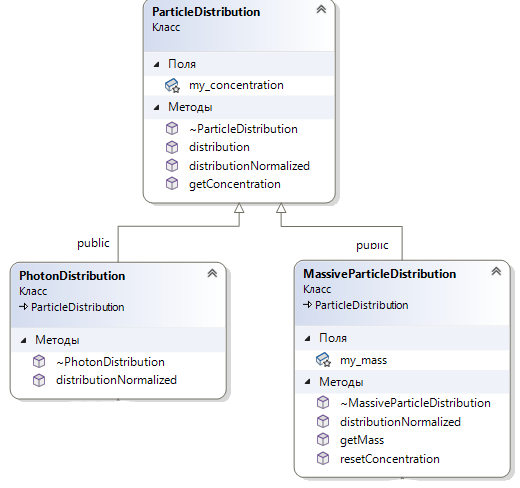
\includegraphics[width=9.5 cm]{./fig/particleDistribution0.png} 
	\caption{Схема наследования распределения фотонов и массивных частиц}
	\label{particleDistribution0}
\end{figure}
Важно отметить, что распределения фотонов не используются для представления результатов расчета излучения. Они нужны как входной параметр для расчета обратного комптоновского рассеяния. Класс PhotonDistribution не имеет дополнительных собственных методов и является лишь интерфейсом. Класс MassiveParticleDistribution тоже является абстрактным, в нем не задан конкретный вид распределения, но добавлены новые методы, описанные в Таблице \ref{MassiveParticleDistribution}	
\begin{table}
	\begin{center}
		\caption{Публичные методы класса MassiveParticleDistribution }
		\label{MassiveParticleDistribution}
		\begin{small}
			\begin{tabularx}{\textwidth}{|X|X|}
				\hline
				\textbf{MassiveParticleDistribution} & \\
				\hline
				getMass() & возвращает массу частиц \\
				\hline
				resetConcentration(const double\& n) & позволяет изменить полную концентрацию частиц в распределении\\
				\hline
			\end{tabularx}
		\end{small}
	\end{center}
\end{table}
\subsection{Распределения фотонов}

От абстрактного класса PhotonDistribution наследуются следующие классы: абстрактный PhotonIsotropicDistribution, предназначенный для представления изотропных распределений фотонов и CompoundPhotonDistribution, представляющий из себя сумму нескольких распределений фотонов общего вида. Схема наследования классов фотонных распределений представлена на рисунке \ref{photonDistribution}.
\begin{figure}
	\centering
	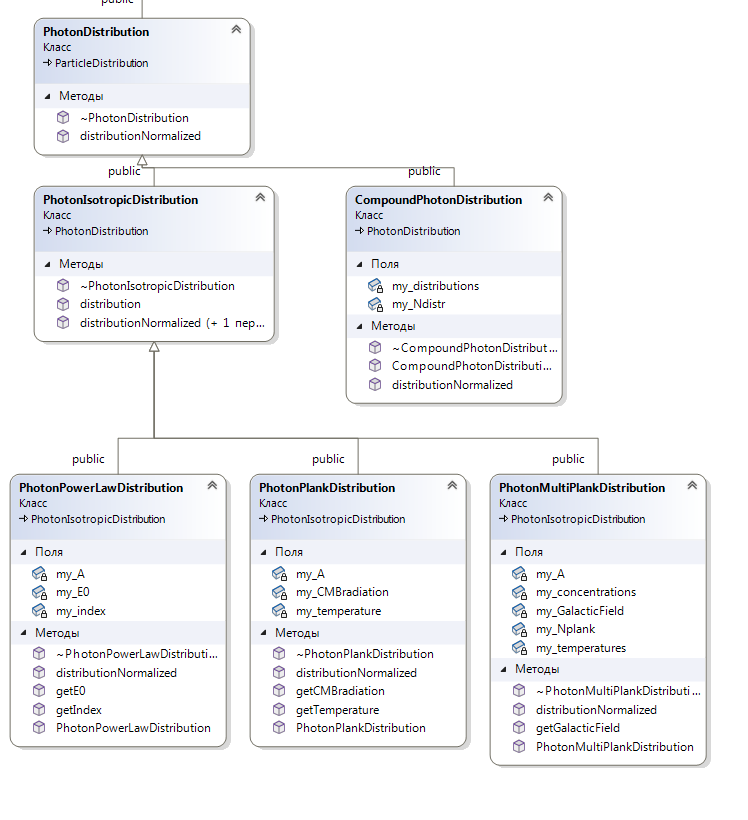
\includegraphics[width=10.5 cm]{./fig/photonDistribution1.png} 
	\caption{Схема наследования классов распределений фотонов}
	\label{photonDistribution}
\end{figure}

У изотропного распределения PhotonIsotropicDistribution добавляются методы, возвращающие значение функции распределения только в зависимости от энергии. Важно понимать, что это не функция распределения по энергии, а полная функция распределения с отброшенными угловыми аргументами. Другими словами, для получения значения функции распределения по энергии нужно домножить значение, возвращенное данным методом на $4 \pi$.

У класса PhotonIsotropicDistribution есть три наследника, которые уже не абстрактные классы, а непосредственно предназначены для создания распределений. Это PhotonPowerLawDistribution для представления степенных распределений, PhotonPlankDistribution, для планковских распределений и PhotonMultiPlankDistribution, для суммы планковских распределений. Метода класса PhotonIsotropicDistribution и его наследников перечислены в таблице \ref{photonDistributionMethods}
\begin{table}[h!]
	\begin{center}
		\caption{Публичные методы классов изотропных распределений фотонов}
		\label{photonDistributionMethods}
		\begin{small}
			\begin{tabularx}{\textwidth}{|X|X|}
				\hline
				\textbf{PhotonIsotropicDistribution} & \\
				\hline
				distribution(const double\& energy) & возвращает функцию распределения с отброшенными угловыми аргументами, то есть нормированную на концентрацию, деленную на $4 \pi$ \\
				\hline
				distributionNormalized(const double\& energy) & возвращает функцию распределения с отброшенными угловыми аргументами, нормированную на  $ 1 / 4 \pi$\\
				\hline
				\textbf{PhotonPowerLawDistribution} & \\
				\hline
				PhotonPowerLawDistribution(const double\& index, const double\& E0, const double\& concentration) & конструктор, создающий экземпляр с заданными показателем наклона, начальной энергией и полной концентрацией \\
				\hline
				getIndex() & возвращает показатель наклона спектра\\
				\hline
				getE0() & возвращает минимальную энергию степенного распределения\\
				\hline
				\textbf{PhotonPlankDistribution} & \\
				\hline
				PhotonPlankDistribution(const double\& temperature, const double\& amplitude) & конструктор, создающий экземпляр с заданными температурой и апмплитудой - то есть отношением концентрации к равновесному планковскому распределению с данной температурой\\
				\hline
				static getCMBRadiation() & статический метод, возвращающий экземпляр, соответствующий реликтовому излучению (температура $2.725 K$, амплитуда $1$)\\
				\hline
				getTemperature() & возвращает температуру распределения\\
				\hline
				\textbf{PhotonMultiPlankDistribution} & \\
				\hline
				PhotonMultiPlankDistribution(int Nplank, const double* const temperatures, const double* const amplitudes) & конструктор, количество планковских распределений, участвующих в смеси, массив их температур и массив амплитуд\\
				\hline
				static getGalacticField() & статический метод, возвращающий экземпляр, соответствующий среднегалактическому фотонному распределению, по данным статьи \cite{Mathis1983}. Данное распределение состоит из пяти планковских компонент, с температурами $2.725K, 20K, 3000K, 4000K, 7000K$ и амплитудами $1.0, 4\cdot10^{4}, 4\cdot10^{-13}, 1.65\cdot10^{-13}, 1.0\cdot10^{-14}$ соответственно\\
				\hline
			\end{tabularx}
		\end{small}
	\end{center}
\end{table}

Класс CompoundPhotonDistribution предназначен для представления смеси различных распределений фотонов, не обязательно планковских, как PhotonMultiPlankDistribution, и не обязательно изотропных. Его методы описаны в Таблице \ref{CompoundPhotonMethods}
\begin{table}
	\begin{center}
		\caption{Публичные методы класса CompoundPhotonDistribution }
		\label{CompoundPhotonMethods}
		\begin{small}
			\begin{tabularx}{\textwidth}{|X|X|}
				\hline
				\textbf{CompoundPhotonDistribution} & \\
				\hline
				CompoundPhotonDistribution(int N, PhotonDistribution** distributions) & конструктор, создающий экземпляр с заданным количеством распределений в смеси и массивом этих распределений \\
				\hline
				CompoundPhotonDistribution( PhotonDistribution* dist1, PhotonDistribution* dist2) & конструктор, создающий экземпляр содержащий смесь из двух распределений\\
				\hline
				CompoundPhotonDistribution( PhotonDistribution* dist1, PhotonDistribution* dist2, PhotonDistribution* dist3) & конструкторб создающий экземпляр содержащий смесь из трех распределений\\
				\hline
			\end{tabularx}
		\end{small}
	\end{center}
\end{table}

Встроенных анизотропных распределений фотонов в коде на данный момент нет, но пользователь может реализовать их самостоятельно, создав класс, наследующий от PhotonDistribution и определив необходимый виртуальный метод distributionNormalized(const double\& energy, const double\& mu, const double\& phi). Аналогично можно, конечно, создать и другие виды изотропных распределений.

\subsection{Распределения массивных частиц}
Распределения массивных частиц представлены наследниками класса MassiveParticleDistribution. Так же как и в случае с фотонами важную роль играет абстрактный клас для представления изотропных распределений - MassiveParticleIsotropicDistribution. У этого класса есть методы возвращающие значение функции распределения в зависимости от энергии, и опять же, это не функция распределения, проинтегрированная по углам, а полная функция распределения с отброшенными угловыми аргументами. Для получения значения функции распределения по энергии нужно домножить значение, возвращенное данным методом на $4 \pi$. Так же добавлен метод записи функции распределения в файл. 

\begin{table}[h!]
	\begin{center}
		\caption{Публичные методы класса MassiveParticleIsotropicDistribution }
		\label{MassiveParticleMethods}
		\begin{small}
			\begin{tabularx}{\textwidth}{|X|X|}
				\hline
				\textbf{MassiveParticleIsotropicDistribution} & \\
				\hline
				distribution(const double\& energy) & возвращает функцию распределения с отброшенными угловыми аргументами, то есть нормированную на концентрацию, деленную на $4 \pi$ \\
				\hline
				distributionNormalized(const double\& energy) & возвращает функцию распределения с отброшенными угловыми аргументами, нормированную на  $ 1 / 4 \pi$\\
				\hline
				writeDistribution(const char* fileName, int Ne, const double\& Emin, const double\& Emax) & записывает распределение в файл с данным именем, в диапазоне межджу данными минимальной и максимальной енергиями с заданным количеством точек, которые распределяются логарифмически\\
				\hline
			\end{tabularx}
		\end{small}
	\end{center}
\end{table}

\begin{figure}[h!]
	\centering
	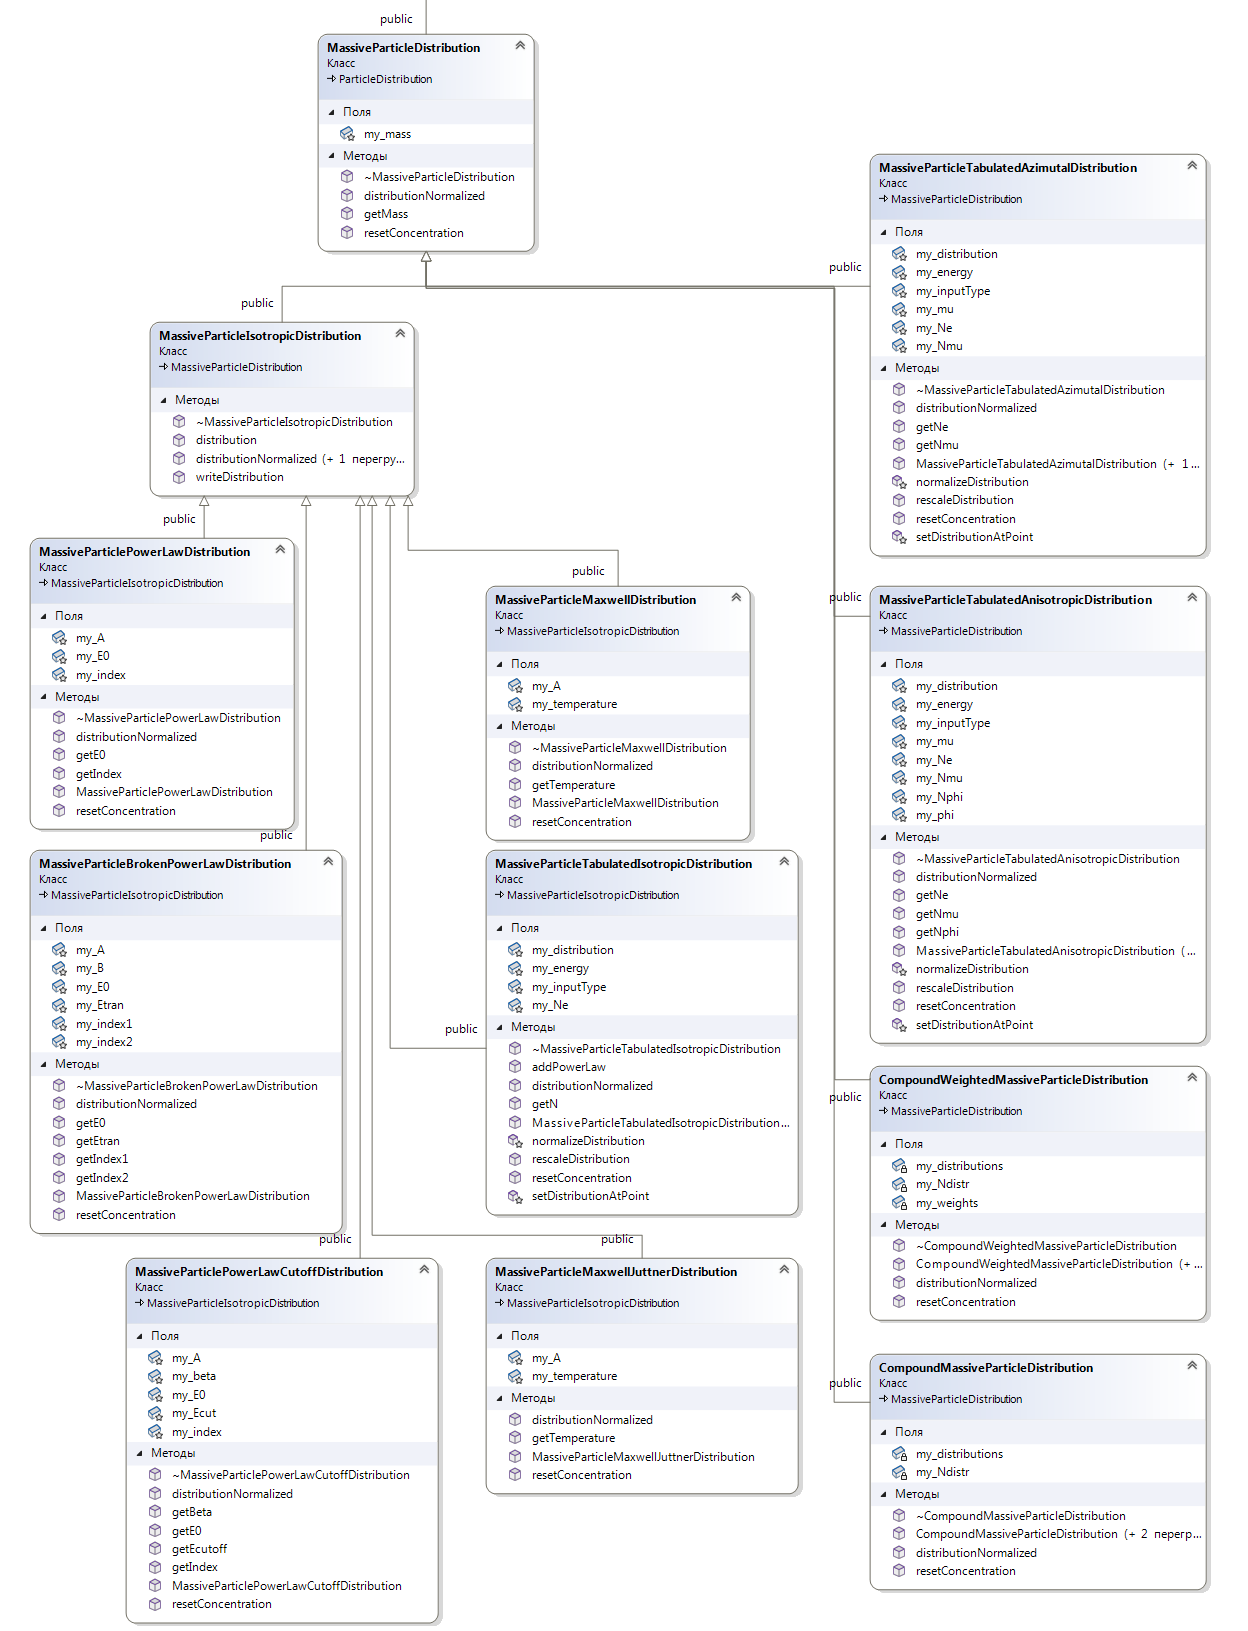
\includegraphics[width=14.5 cm]{./fig/massiveParticleDistribution1.png} 
	\caption{Схема наследования классов распределения массивных частиц}
	\label{massiveDistribution}
\end{figure}

Абстрактный класс изотропных распределений имеет шесть наследников, предназначенных для создания конкретных распределений: MassiveParticlePowerLawDistribution - для степенных распределений, MassiveParticleBrokenPowerLawDistribution - для степенных распределений с изломом, MassiveParticlePowerLawCutoffDistribution - для степенных распределений с экспоненциальным завалом, MassiveParticleMaxwellDistribution - для максвелловского распределения (обратите внимание, что в отличие от остальных распределений, максвелловское подразумевает под энергией только кинетическую энергию), MassiveParticleMaxwellJuttnerDistribution - для релятивистского распределения Максвелла-Юттнера и MassiveParticleTabulatedIsotropicDistribution - для таблично заданных распределений. 

Так же имеется четыре реализации анизотропных распределений: MassiveParticleTabulatedPolarDistribution - для таблично заданных распределений с зависимостью только от энергии и полярного угла, MassiveParticleAnisotropicDistribution - для таблично заданных распределений с зависимостью от всех переменных, CompoundMassiveParticleDistribution - для суммы распредлений общего вида, CompoundWeightedMassiveParticleDistribution - для взвешенной суммы распределений общего вида. В некоторых случаях оперировать весами распределений удобнее, чем непосредственно концентрациями. Полная схема наследования классов распределений массивных частиц представлена на рисунке \ref{massiveDistribution}, список публичных методов классов распределений массивных частиц приведен в Таблице \ref{MassiveParticleMethods1}. Пользователь может сам реализовывать необходимые ему виды распределений излучающих частиц, создав наследника класса MassiveParticleDistribution или MassiveParticleIsotropicDistribution и определив необходимые виртуальные методы.

\subsection{Считывание распределений из файла}
Классы таблично-заданных распределений, такие как например MassiveParticleTabulatedIsotropicDistribution, имеют конструктор принимающие на вход имена файлов, из которых будет считана функция распределения. Это должны быть текстовые файлы, содержащие таблицы с данными, причем формат единиц, в которых измеряется функция распределения может быть разным. Для задания формата входных файлов используется перечислимы тип DistributionInputType, имеющий пять значений:

\begin{itemize}
	\item ENERGY\_FE - во входных файлах заданы энергия и функция распределения по энергии
	\item ENERGY\_KIN\_FE - заданы кинетическая энергия и функция распределения по энергии
	\item GAMMA\_FGAMMA - задан лоренц-фактор и функция распределения по нему
	\item GAMMA\_KIN\_FGAMMA - задан лоренц-фактор, уменьшенный на единицу, и функция распределения по нему
	\item MOMENTUM\_FP - задан импульс и функция распределения по импульсу
\end{itemize}

Вне зависимости от формата входного файла, функция распределения будет преобразована к единицам энергия - распределение по энергии. С помощью этих параметров можно считывать табличные распределения из файлов, например так:
\begin{lstlisting}[language=c++]
	double electronConcentration = 1.0;
	int N = 100;
	MassiveParticleIsotropicDistribution* distribution = new
	MassiveParticleTabulatedIsotropicDistribution(massElectron,
	"energy.dat", "distribution.dat", N, electronConcentration,
	DistributionInputType::ENERGY_FE);
\end{lstlisting}

Для облегчения создания распределений из файла в сложных случаях реализован класс MassiveParticleDistributionFactory. У него есть несколько методов, позволяющих считывать целые серии распределений из набора пронумерованных файлов. Что может быть полезно, если функция распределения зависит от некоторого параметра, как в примере вычисления синхротронного излучения описанном в следующей главе \ref{}. Считать серию из десяти распределений электронов, содержащихся в файлах с именами  "Fe0.dat"\ , "Fe1.dat"\  и так далее, состоящих из двух колонок - лоренц-фактор и функция распределения, и добавить к этим распределениям степенной хвост с показателем 3, начиная с энергий в 100 энергий покоя можно вызовом одной функции: 

\begin{lstlisting}[language=c++]
	double electronConcentration = 1.0;
	int Nenergy = 100;
	int Ndistribution = 100;
	double powerLawEnergy = 100*me_c2;
	double index = 3.0;
	MassiveParticleIsotropicDistribution** distributions = 
	MassiveParticleDistributionFactory::
	readTabulatedIsotropicDistributionsAddPowerLawTail(
	massElectron, "./input/Fe", ".dat", Ndistribution, 
	DistributionInputType::GAMMA_FGAMMA, electronConcentration, Nenergy,
	powerLawEnergy, index);
\end{lstlisting}

Так же у пользователя есть возможность использовать конструкторы табличных распределений, принимающие не имена файлов, а непосредственно массивы со значениями функции распределения, которые пользователь создать любым удобным ему способом.

\begin{small}
	\topcaption{Публичные методы классов распределений массивных частиц }
	\label{MassiveParticleMethods1}
	\begin{xtabular}{|p{0.52\textwidth}|p{0.48\textwidth}|}
		\hline
		\textbf{MassiveParticlePowerLawDistribution} & \\
		\hline
		MassiveParticlePowerLawDistribution( const double\& mass, const double\& index, const double\& E0, const double\& concentration) & конструктор, создает экземпляр степенного распределния частиц с заданными массой, степенным индексом, начальной энергией распределения и полной концентрацией\\
		\hline
		getIndex() & возвращает степенной индекс распределения\\
		\hline
		getE0() & возвращает начальную энергию распределения\\
		\hline
		\textbf{MassiveParticleBrokenPowerLawDistribution} & \\
		\hline
		MassiveParticleBrokenPowerLawDistribution( const double\& mass, const double\& index1, const double\& index2, const double\& E0, const double\& Etran, const double\& concentration) & конструктор, создает экземпляр степенного распределния с изломом частиц с заданными массой, степенными индексоми на низких и высоких энергиях, начальной энергией распределения, энергией соответствующей излому и полной концентрацией\\
		\hline
		getIndex1() & возвращает степенной индекс распределения на низких энергиях\\
		\hline
		getIndex2() & возвращает степенной индекс распределения на высоких энергиях\\
		\hline
		getE0() & возвращает начальную энергию распределения\\
		\hline
		getEtran() & возвращает энергию излома\\
		\hline
		\textbf{MassiveParticlePowerLawCutoffDistribution} & \\
		\hline
		MassiveParticlePowerLawCutoffDistribution(const double\& mass, const double\& index, const double\& E0, const double\& beta, const double\& Ecut, const double\& concentration) & конструктор, создает экземпляр степенного распределния с экспоненциальным завалом частиц с заданными массой, степенным индексом, начальной энергией распределения, параметром завала, энергией завала и полной концентрацией. $F(E)\propto (E/E_0)^{-index}\cdot\exp(-(E/E_{cut})^\beta)$\\
		\hline
		getIndex() & возвращает степенной индекс распределения \\
		\hline
		getBeta() & возвращает параметр завала распределения \\
		\hline
		getE0() & возвращает начальную энергию распределения\\
		\hline
		getEcutoff() & возвращает энергию экспоненциального завала\\
		\hline
		\textbf{MassiveParticleMaxwellDistribution} & \\
		\hline
		MassiveParticleMaxwellDistribution( const double\& mass, const double\& temperature, const double\& concentration) & конструктор, создает экземпляр распределния Максвелла частиц с заданными массой, температурой и полной концентрацией\\
		\hline
		getTemperature() & возвращает температуру распределения\\
		\hline
		\textbf{MassiveParticleMaxwellJuttnerDistribution} & \\
		\hline
		MassiveParticleMaxwellJuttnerDistribution( const double\& mass, const double\& temperature, const double\& concentration) & конструктор, создает экземпляр распределния Максвелла-Юттнера частиц с заданными массой, температурой и полной концентрацией\\
		\hline
		getTemperature() & возвращает температуру распределения\\
		\hline
		\textbf{MassiveParticleTabulatedIsotropicDistribution} & \\
		\hline
		MassiveParticleTabulatedIsotropicDistribution( const double\& mass, const char* fileName, const int N, const double\& concentration, DistributionInputType inputType) & конструктор, создает экземпляр табличного распределния частиц с заданными массой и полной концентрацией с помощью указанного файла, состоящего из двух колнок с данными указанной длины. Так же указывается формат входных данных.\\
		\hline
		MassiveParticleTabulatedIsotropicDistribution( const double\& mass, const char* energyFileName, const char* distributionFileName, const int N, const double\& concentration, DistributionInputType inputType) & конструктор, создает экземпляр табличного распределния частиц с заданными массой и полной концентрацией с помощью указанных двух файлов, состоящих из колнок с данными указанной длины. Так же указывается формат входных данных. \\
		\hline
		MassiveParticleTabulatedIsotropicDistribution( const double\& mass, const double* energy, const double* distribution, const int N, const double\& concentration, DistributionInputType inputType) & конструктор, создает экземпляр табличного распределния частиц с заданными массой и полной концентрацией с помощью двух переданных массивов данных указанной длины. Так же указывается формат входных данных.\\
		\hline
		getN() & возвращает количество ячеек в таблице задающей функцию\\
		\hline
		getEmin() & возвращает минимальную энергию распределения\\
		\hline
		getEmax() & возвращает максимальную энергию распределения\\
		\hline
		rescaleDistribution(const double\& k) & масштабирует распределение, вытягивая его по оси энергии по формуле $E' = mc^2 + k\cdot(E-mc^2)$, $F(E')=F(E)/k$. Данная функция может быть полезна, например, в случае когда исходная функция распределения получена в результате работы численного кода с измененной массой электронов\\
		\hline
		addPowerLaw( const double\& Epower, const double\& index) & добавляет к функции распределения степенной с указанным индексом, начиная с указанной энергии. Функция распределения при этом остается нормированной на указанную ранее концентрацию\\
		\hline 
		\textbf{MassiveParticleTabulatedPolarDistribution} & \\
		\hline
		MassiveParticleTabulatedPolarDistribution( const double\& mass, const char* energyFileName, const char* muFileName, const char* distributionFileName, const int Ne, const int Nmu, const double\& concentration, DistributionInputType inputType) & конструктор, создает экземпляр табличного распределния частиц с заданными массой и полной концентрацией с помощью  трех указанных файлов, в двух из которых содержатся сетки по энергии и косинусу полярного угла с указанными размерами, а в третьем двумерный массив функции распределения. Так же указывается формат входных данных.\\
		\hline
		MassiveParticleTabulatedPolarDistribution( const double\& mass, const double* energy, const double* mu, const double** distribution, const int Ne, const int Nmu, const double\& concentration, DistributionInputType inputType) & конструктор, создает экземпляр табличного распределния частиц с заданными массой и полной концентрацией с помощью трех переданных массивов данных, в двух из которых содержатся сетки по энергии и косинусу полярного угла с указанными размерами, а в третьем двумерный массив функции распределения. Так же указывается формат входных данных.\\
		\hline
		getNe() & возвращает количество ячеек по энергии в таблице задающей функцию распределения\\
		\hline
		getEmin() & возвращает минимальную энергию распределения\\
		\hline
		getEmax() & возвращает максимальную энергию распределения\\
		\hline
		getNmu() & возвращает количество ячеек по полярному углу в таблице задающей функцию распределения\\
		\hline
		rescaleDistribution(const double\& k) & масштабирует распределение, вытягивая его по оси энергии по формуле $E' = mc^2 + k\cdot(E-mc^2)$, $F(E',\mu)=F(E,\mu)/k$. Данная функция может быть полезна, например, в случае когда исходная функция распределения получена в результате работы численного кода с измененной массой электронов\\
		\hline
		\textbf{MassiveParticleTabulatedAnisotropicDistribution} & \\
		\hline
		MassiveParticleTabulatedAnisotropicDistribution( const double\& mass, const char* energyFileName, const char* muFileName, const char* distributionFileName, const int Ne, const int Nmu, const int Nphi, const double\& concentration, DistributionInputType inputType) & конструктор, создает экземпляр табличного распределния частиц с заданными массой и полной концентрацией с помощью  трех указанных файлов, в двух из которых содержатся сетки по энергии и косинусу полярного угла с указанными размерами, а в третьем двумерный массив функции распределения. Сетка по азимутальному углу считается расномерной и определяется только размером. Так же указывается формат входных данных.\\
		\hline
		MassiveParticleTabulatedAnisotropicDistribution( const double\& mass, const double* energy, const double* mu, const double*** distribution, const int Ne, const int Nmu, const int Nphi, const double\& concentration, DistributionInputType inputType) & конструктор, создает экземпляр табличного распределния частиц с заданными массой и полной концентрацией с помощью трех переданных массивов данных, в двух из которых содержатся сетки по энергии и косинусу полярного угла с указанными размерами, а в третьем двумерный массив функции распределения. Сетка по азимутальному углу считается расномерной и определяется только размером. Так же указывается формат входных данных.\\
		\hline
		getNe() & возвращает количество ячеек по энергии в таблице задающей функцию распределения\\
		\hline
		getEmin() & возвращает минимальную энергию распределения\\
		\hline
		getEmax() & возвращает максимальную энергию распределения\\
		\hline
		getNmu() & возвращает количество ячеек по полярному углу в таблице задающей функцию распределения\\
		\hline
		getNphi() & возвращает количество ячеек по азимутальному углу в таблице задающей функцию распределения\\
		\hline
		rescaleDistribution(const double\& k) & масштабирует распределение, вытягивая его по оси энергии по формуле $E' = mc^2 + k\cdot(E-mc^2)$, $F(E',\mu, \phi)=F(E,\mu, \phi)/k$. Данная функция может быть полезна, например, в случае когда исходная функция распределения получена в результате работы численного кода с измененной массой электронов\\
		\hline
		\textbf{CompoundMassiveParticleDistribution} & \\
		\hline
		CompoundMassiveParticleDistribution( int N, MassiveParticleDistribution** distributions) & конструктор, создает экземпляр класса содержащий смесь заданного количества указанных распределений\\
		\hline
		CompoundMassiveParticleDistribution( MassiveParticleDistribution* dist1, MassiveParticleDistribution* dist2) & конструктор, создает экземпляр класса, содержащий смесь двух распределений \\
		\hline
		CompoundMassiveParticleDistribution( MassiveParticleDistribution* dist1, MassiveParticleDistribution* dist2, MassiveParticleDistribution* dist3) & конструктор, создает экземпляр класса, содержащий смесь трех распределений\\
		\hline
		\textbf{CompoundWeightedMassiveParticleDistribution} & \\
		\hline
		CompoundWeightedMassiveParticleDistribution( int N, const double* weights, MassiveParticleDistribution** distributions) & конструктор, создает экземпляр класса содержащий смесь заданного количества указанных распределений с заданными весами \\
		\hline
		CompoundWeightedMassiveParticleDistribution( MassiveParticleDistribution* dist1, const double\& w1, MassiveParticleDistribution* dist2, const double\& w2) & конструктор, создает экземпляр класса, содержащий смесь двух распределений с указанными весами \\
		\hline
		CompoundWeightedMassiveParticleDistribution( MassiveParticleDistribution* dist1, const double\& w1, MassiveParticleDistribution* dist2, const double\& w2, MassiveParticleDistribution* dist3, const double\& w3) & конструктор, создает экземпляр класса, содержащий смесь трех распределений с указанными весами \\
		\hline
				
	\end{xtabular}
\end{small}

